\documentclass[]{scrartcl}
\usepackage{graphicx}
\usepackage{color}
\usepackage{hyperref}
\usepackage{calc} 
\usepackage{enumitem}
\newcommand{\source}[1]{\vspace{-3pt} \caption*{ Source: {#1}} }
%\pagestyle{headings}

% customize dictum format:
\usepackage[T1]{fontenc}
\setkomafont{dictumtext}{\itshape\small}
\setkomafont{dictumauthor}{\normalfont}
\renewcommand*\dictumwidth{\linewidth}
\renewcommand*\dictumauthorformat[1]{--- #1}
\renewcommand*\dictumrule{}
\newcommand{\todo}[1]{\textcolor{red}{TODO: #1}\PackageWarning{TODO:}{#1!}}

\begin{document}

\title{
	\includegraphics*[width=0.63\textwidth]{images/yale_logo.png}\\
	\vspace{24pt}
	ENGL 300:\\Introduction to Theory of Literature}
\subtitle{Lecture Spring, 2009\\
          Paul H. Fry\\
          William Lampson Professor of English \\ 
          Yale University}
\author{Lennard Wolf\\
        \href{mailto:lennard.wolf@student.hu-berlin.de}{lennard.wolf@student.hu-berlin.de}}
\maketitle
\begin{abstract}

This is a survey of the main trends in twentieth-century literary theory. Lectures will provide background for the readings and explicate them where appropriate, while attempting to develop a coherent overall context that incorporates philosophical and social perspectives on the recurrent questions: what is literature, how is it produced, how can it be understood, and what is its purpose?

\end{abstract}
\newpage

\tableofcontents

\listoffigures
\newpage


\section{Introduction I}


\subsection{Description Text}
\dictum[William Wordsworth, \textit{The Friend, 1805}]{%
Bliss was it in that dawn to be alive}
\vspace{15pt}

In this first lecture, Professor Paul Fry explores the course's title in three parts. The relationship between theory and philosophy, the question of what literature is and does, and what constitutes an introduction are interrogated. The professor then situates the emergence of literary theory in the history of modern criticism and, through an analysis of major thinkers such as Marx, Nietzsche, and Freud, provides antecedents for twentieth-century theoretical developments.

\subsection{Content}
\dictum[Georg Wilhelm Friedrich Hegel, \textit{Die Vernunft in der Geschichte}]{%
Was der Geist will, ist, seinen eigenen Begriff erreichen (den Ort an dem er theoretisch und praktisch in Harmonie mit dem Ganzen steht); aber er selbst verdeckt sich denselben, ist stolz und voll Genu\ss~in dieser Entfremdung seiner selbst.}
\vspace{15pt}

Literature can not really be defined clearly, as exceptions to the rule always persist. However defining it helps us deal with complexity, and to understand what literature is, is in part goal of this lecture. \emph{Theory} has the goal of analyzing the text to for example understand its meaning and can thus be put to practice using certain methodologies. Questions raised by Literary Theory can be \emph{"What is a reader/an author?"} etc.

Scepticism has its roots in \emph{Modernity} (generation of Descartes, Shakespeare, and Cervantes), with thinkers starting to question common assumptions (like Descartes in his \emph{Meditations}: \emph{"Well, might I not be crazy?"}). In 1796, Kant further questioned the relationship of our knowledge of the world with its reality (\emph{"We cannot know the thing in itself."}). Then, in his 1807 book \emph{The Phenomenology of Mind}, Hegel says that these developments in thought have formed a sort of \emph{Entfremdung}, through which we are driven away from our goal to know ourselves.

Modern skepticism has three central figures: Marx, Nietzsche, and Freud. Their core thoughts which are relevant here are the following:

\begin{description}[leftmargin=!,labelwidth=\widthof{\bfseries Nietzsche}]
  \item[Marx] In \emph{Kapital}, M. talks about \emph{commodity fetishism}, through which we assign "objective" value to commodities, such as human labor. He then compares commodity fetishism to the belief in God, stating that both are determined by social, historical, and economic factors, and are both part of \textbf{ideology}, which the ideologically thinking person can not escape.
  \item[Nietzsche] For N., the underpinnings of consciousness which make the operations of consciousness inauthentic are the nature of \textbf{language} itself. "\emph{What then is truth? A mobile army of metaphors, metonymies, anthropomorphisms--in short, a sum of human relations which became poetically and rhetorically intensified,}" etc., etc., etc., "\emph{and are now no longer of account as coins but are debased.}". However, N. believed that once there was a moment in language time, were that was not the case and only truth was said.
  \item[Freud] In \emph{The Psychopathology of Everyday Life}, F. says that after all, we have absolutely no objective evidence that the unconscious exists. If I could see the unconscious, it'd be conscious. The unconscious is something that we have to infer from the way consciousness operates. We've got to figure out somehow how it is that consciousness is never completely uninhibited, never completely does and says what it wants to say. So the spin on consciousness for Freud is the \textbf{unconscious}.
  
\end{description}

Now, we do not only have no knowledge of ourselves, but also none about the objects around us and their relationship with us. This has perplexed many people, and so many large, angry volumes were written against such skepticism and the literary theory that it had sparked.

\subsection{New Words}

\begin{description}[leftmargin=!,labelwidth=\widthof{\bfseries Cartesian Revolution}]
  \item[Literature] Literature can not really be defined clearly, as exceptions to the rule always persist. Thus definitions of literature can always only exist in a certain context.
  \item[Hermeneutics] The science of interpreting and understanding of human symbols, usually in the form of text.
  \item[Literary Theory] In contrast to \emph{Literary Criticism}, Literary Theory is not concerned with opinionating and defining the value of a text, but rather with systematically analyzing and dwelling on it, while considering history, philosophy, and other fields which are relevant to the interpretation of meaning. Today, it is often referred to as \emph{Theory} in the academic world.
  \item[Modernity] (Not to be confused with \emph{Modernism}, which is a more nuanced cultural movement in late Modernity) Coined by Baudelaire in his essay \emph{The Painter of Modern Life}. Historical period (1453 - 1989), in which first through art and later all other sciences tradition is more and more questioned and rejected. Individualism, freedom, and formal equality are key values.
  \item[Cartesian Revolution] Begin of rationalist thought after Descartes
  \item[Verfremdung] ??
\end{description}

\section{Introduction II}

\subsection{Description Text}

\dictum[Immanuel Kant, \textit{Reflexionen}]{%
Er ist ein Egoist der Wissenschaft, und es ist ihm noch ein Auge n\"otig, welches macht, dass er seinen Gegenstand noch aus dem Gesichtspunkte anderer Menschen ansieht...}
\vspace{15pt}

In this second introductory lecture, Professor Paul Fry explores the interrelation of skepticism and determinism. The nature of discourse and the related issue of \emph{discursivity} is read through two modern works, Anton Chekov's \emph{Cherry Orchard} and Henry James' \emph{The Ambassadors}. Exemplary critical focus on literary authority is located in Michel Foucault's \emph{What Is an Author} and Roland Barthes' \emph{The Death of the Author}, both of which are read with an emphasis on their historical contexts. Objections to the approach and conclusions of the two theorists are examined, particularly in light of the rise of cultural studies.

\subsection{Content}

\dictum[Henry James, \textit{The Ambassadors}]{%
Don't do what I have done. Don't miss out on life. Live all you can. It is a mistake not to. And this is why, the affair, I mean the affair of life couldn't, no doubt, have been different for me for it's at the best a tin mold either fluted or embossed with ornamental excrescences or else smooth and dreadfully plain, into which, a helpless jelly, one's consciousness, is poured so that one takes the form, as the great cook says, and is more or less compactly held by it. One lives, in fine, as one can. Still one has the illusion of freedom.}
\vspace{15pt}



The aftermath of skepticism was not only the question of how we can know things in themselves, but also, how can we trust the \textbf{autonomy} of someone, who believes to know something. Such hidden forces (e.g. \textbf{determinism}) were also mentioned in the work of Darwin, who posed the question on \emph{human agency}, of what may become of the idea of human autonomy. Or more bluntly: \emph{Are we actually autonomous?} The following two literary examples from the early 20th century illustrate this bother:

\begin{description}[leftmargin=!,labelwidth=\widthof{\bfseries The Ambassadors}]
  \item[Cherry Orchard] In Chekov's book, an autodidact house servant (low class) pities his situation and wonders about the determinism behind his fate on both the level of being born into his situation, as well as language, in the way that it determines his thinking. This debased situation (reminds me of Heidegger) he finds himself in is derived from Hamlet.
  \item[The Ambassadors] James's book revolves around a young man who is supposed to take over his family's business, but who has awakened to the wonder of urbane culture. He says to a young man at a party: "\emph{Therefore, don't be like me without the memory of that illusion. I was either at the right time too stupid or too intelligent to have it. I don't quite know which.}" Too stupid referring to Nietzsches \emph{historical man}, the one who would plunge into life without looking left nor right, and too intelligent meaning to be unable to bear the knowledge that freedom is an illusion.
\end{description}

These two accounts introduce the theme of the \textbf{loss of authority} or authorship and let us jump to the end of the 60's in Paris, where students and professors were out protesting on the street, questioning and resisting authority. In those times, Jacques Foucault wrote his essay \emph{What is an author?}, in which he describes the author as a \emph{function}, rather than a person. This \emph{author-function} is a sort of signal in the text, which can raise the question of where and what the author actually is (see the Barthes quotes in the New Word section). 

This can be exemplified by a habit of students of the Johns Hopkins University in the 60's, where they would raise their arms during lectures of Poulet and simply say an author's name, to which Poulet would respond "\emph{Mais, oui! Exactement! A mon avis aussi!}". Here, the authors' names were not referring to the persons by themselves, but rather their oeuvres and fields of \textbf{discursivity}. \emph{Discourse} here is academic jargon for a delimited and structured field of thought or theory. In such a field, meaning of a word can differ from a different field, and so more clear communication can happen. While Foucault holds that the author-function is still an aspect to deciphering a text, Barthes says that the text is a \emph{structure becomes so complex, that is ceases to be a structure}, and so the author-function is just a bit in the matrix of the text. To give a text an author limits the text and closes it, opening it up to \textbf{policing of meaning} and critique.

However there of course are many people who object to the notion of the author-function, and think that it is still important to rate authors and pay hommage, to value their creativity and importance. Furthermore, Foucault himself often speaks of and cites "Marx" and "Freud", how can he do this without accepting their authority? To answer this, he introduces a new concept: instead of \emph{author}, they are \emph{founders of discursivity}, which is why we today say a text is \emph{freudian}.

A consequence of this disappearance of the author is, according to Foucault, that the author is no legal status, and thus intellectual property also ceases to exist. This is, again, objected by proponents of identity politics in cultural studies, to which autonomous identity is both weapon and part of the goal in the fight for freedom.

\subsection{New Words}

\dictum[Roland Barthes, \textit{S/Z}]{%
Who is speaking thus? Is it the hero of the story, [...] Balzac the author, [...] universal wisdom? Romantic psychology? We shall never know, for the good reason that writing is the destruction of every voice, of every point of origin.
}
\vspace{15pt}


\begin{description}[leftmargin=!,labelwidth=\widthof{\bfseries Proliferation}]
  \item[Agency] The capacity of an actor (a person or other entity, human or any living being in general, or soul-consciousness in religion) to act in any given environment (e.g. a social structure).
  \item[Precocious] Altklug; Naseweis; Fr\"uhreif.
  \item[Futile] Zwecklos.
  \item[Proliferation] Rapid increase in numbers. Vermehrung
  \item[Genealogy] ???
\end{description}

\section{Ways In and Out of the Hermeneutic Circle}

\dictum[Immanuel Kant, \textit{Reflexionen}]{%
Er ist ein Egoist der Wissenschaft, und es ist ihm noch ein Auge n\"otig, welches macht, dass er seinen Gegenstand noch aus dem Gesichtspunkte anderer Menschen ansieht...}
\vspace{15pt}

\subsection{Description Text}

\subsection{Content}

\begin{itemize}
\item more work
\item more responsibility
\item more satisfaction
\end{itemize}


\subsection{New Words}

\begin{description}[leftmargin=!,labelwidth=\widthof{\bfseries Cartesian Revolution}]
  \item[Literature] asdf
\end{description}

\section{Configurative Reading}

\dictum[Immanuel Kant, \textit{Reflexionen}]{%
Er ist ein Egoist der Wissenschaft, und es ist ihm noch ein Auge n\"otig, welches macht, dass er seinen Gegenstand noch aus dem Gesichtspunkte anderer Menschen ansieht...}
\vspace{15pt}

\subsection{Description Text}


\subsection{Content}

\begin{itemize}
\item more work
\item more responsibility
\item more satisfaction
\end{itemize}


\subsection{New Words}

\begin{description}[leftmargin=!,labelwidth=\widthof{\bfseries Cartesian Revolution}]
  \item[Literature] asdf
\end{description}

\section{Ways In and Out of the Hermeneutic Circle}

\dictum[Immanuel Kant, \textit{Reflexionen}]{%
Er ist ein Egoist der Wissenschaft, und es ist ihm noch ein Auge n\"otig, welches macht, dass er seinen Gegenstand noch aus dem Gesichtspunkte anderer Menschen ansieht...}
\vspace{15pt}

\subsection{Description Text}


\subsection{Content}

\begin{itemize}
\item more work
\item more responsibility
\item more satisfaction
\end{itemize}


\subsection{New Words}

\begin{description}[leftmargin=!,labelwidth=\widthof{\bfseries Cartesian Revolution}]
  \item[Literature] asdf
\end{description}

\newpage





\section{Meta}
\subsection{The Professor}
Prof. Paul H. Fry (see Figure \ref{fig:paul_fry}) received his B.A. from University of California, Berkeley in 1966 and earned his Ph.D. in 1973 from Harvard University, where he had writ7ten his dissertation \emph{"Byron’s Myth of the Self"}. He has taught at Yale University since 1971, became Assistant Professor of English in 1973, Associate Professor of English in 1979, Professor of English in 1985 and William Lampson Professor of English in 1993.

\begin{figure}[]
	\centering
	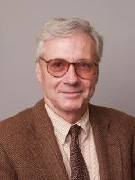
\includegraphics[width=0.32\textwidth]{images/paul_fry.jpg}
	\caption{Prof. Paul Fry. Source: \url{https://www.library.yale.edu/judaica/site/conferences/Amichai/Speaker\%20pics/roundtable/Fry_1051.jpg}}
	\label{fig:paul_fry}
\end{figure}

\subsection{Texts}

Richter, David, ed. The Critical Tradition, 3rd ed. (Bedford-St. Martin's, 2006)


\end{document}
